\chapter{Evaluation}\label{ch:eval}
%Every job in our field includes a performance evaluation. This chapter should show which methods have been used to evaluate performance and what results have been achieved. It is important not only to provide the reader with some figures, but also to discuss the results. It is very good if you first discuss and make plausible what results you expect and then discuss possible deviations. (up to 10 pages)

The design was evaluated in multiple steps to assess the impact of specific design decisions. To expedite the testing cycle, a smaller prototype comprising only 32,768 units was utilized, reducing the compilation time from over 10 hours to approximately 45 minutes. This smaller prototype employs the same techniques as the larger design, but it is decomposed into 256- and 128-point kernels. The evaluation focused on both runtime and precision metrics. For an accurate analysis, the runtime was measured separately for the \ac{pl} and the AI Engines. Given that the primary focus of this work is on the AI Engines, they are expected to perform significantly better than the \ac{pl}.\par

%TODO change name to test case or something else more appropriate
\section{Benchmark setup}
For the aforementioned analysis, various measurements are required. These measurements are conducted using the XRT driver described in section \ref{sec:aie_im}. The start and stop points of the measurements are illustrated in figure \ref{fig:timing}. As shown, all measurements commence and conclude either before or after data is written to the main memory. This approach is taken because the DDR access times are not considered part of the algorithm. In practice, the data is expected to originate from one of the various I/O streaming ports and will be sent there for further processing. The \ac{cpu} and DDR are not involved in this process. Additionally, it is important to note that each component of the algorithm is measured separately, and one comprehensive measurement is performed for a complete run of all components. To ensure reliable results, each measurement is repeated 10 times, and the mean value of the results is calculated.\par

\begin{figure}[h]
    \centering
    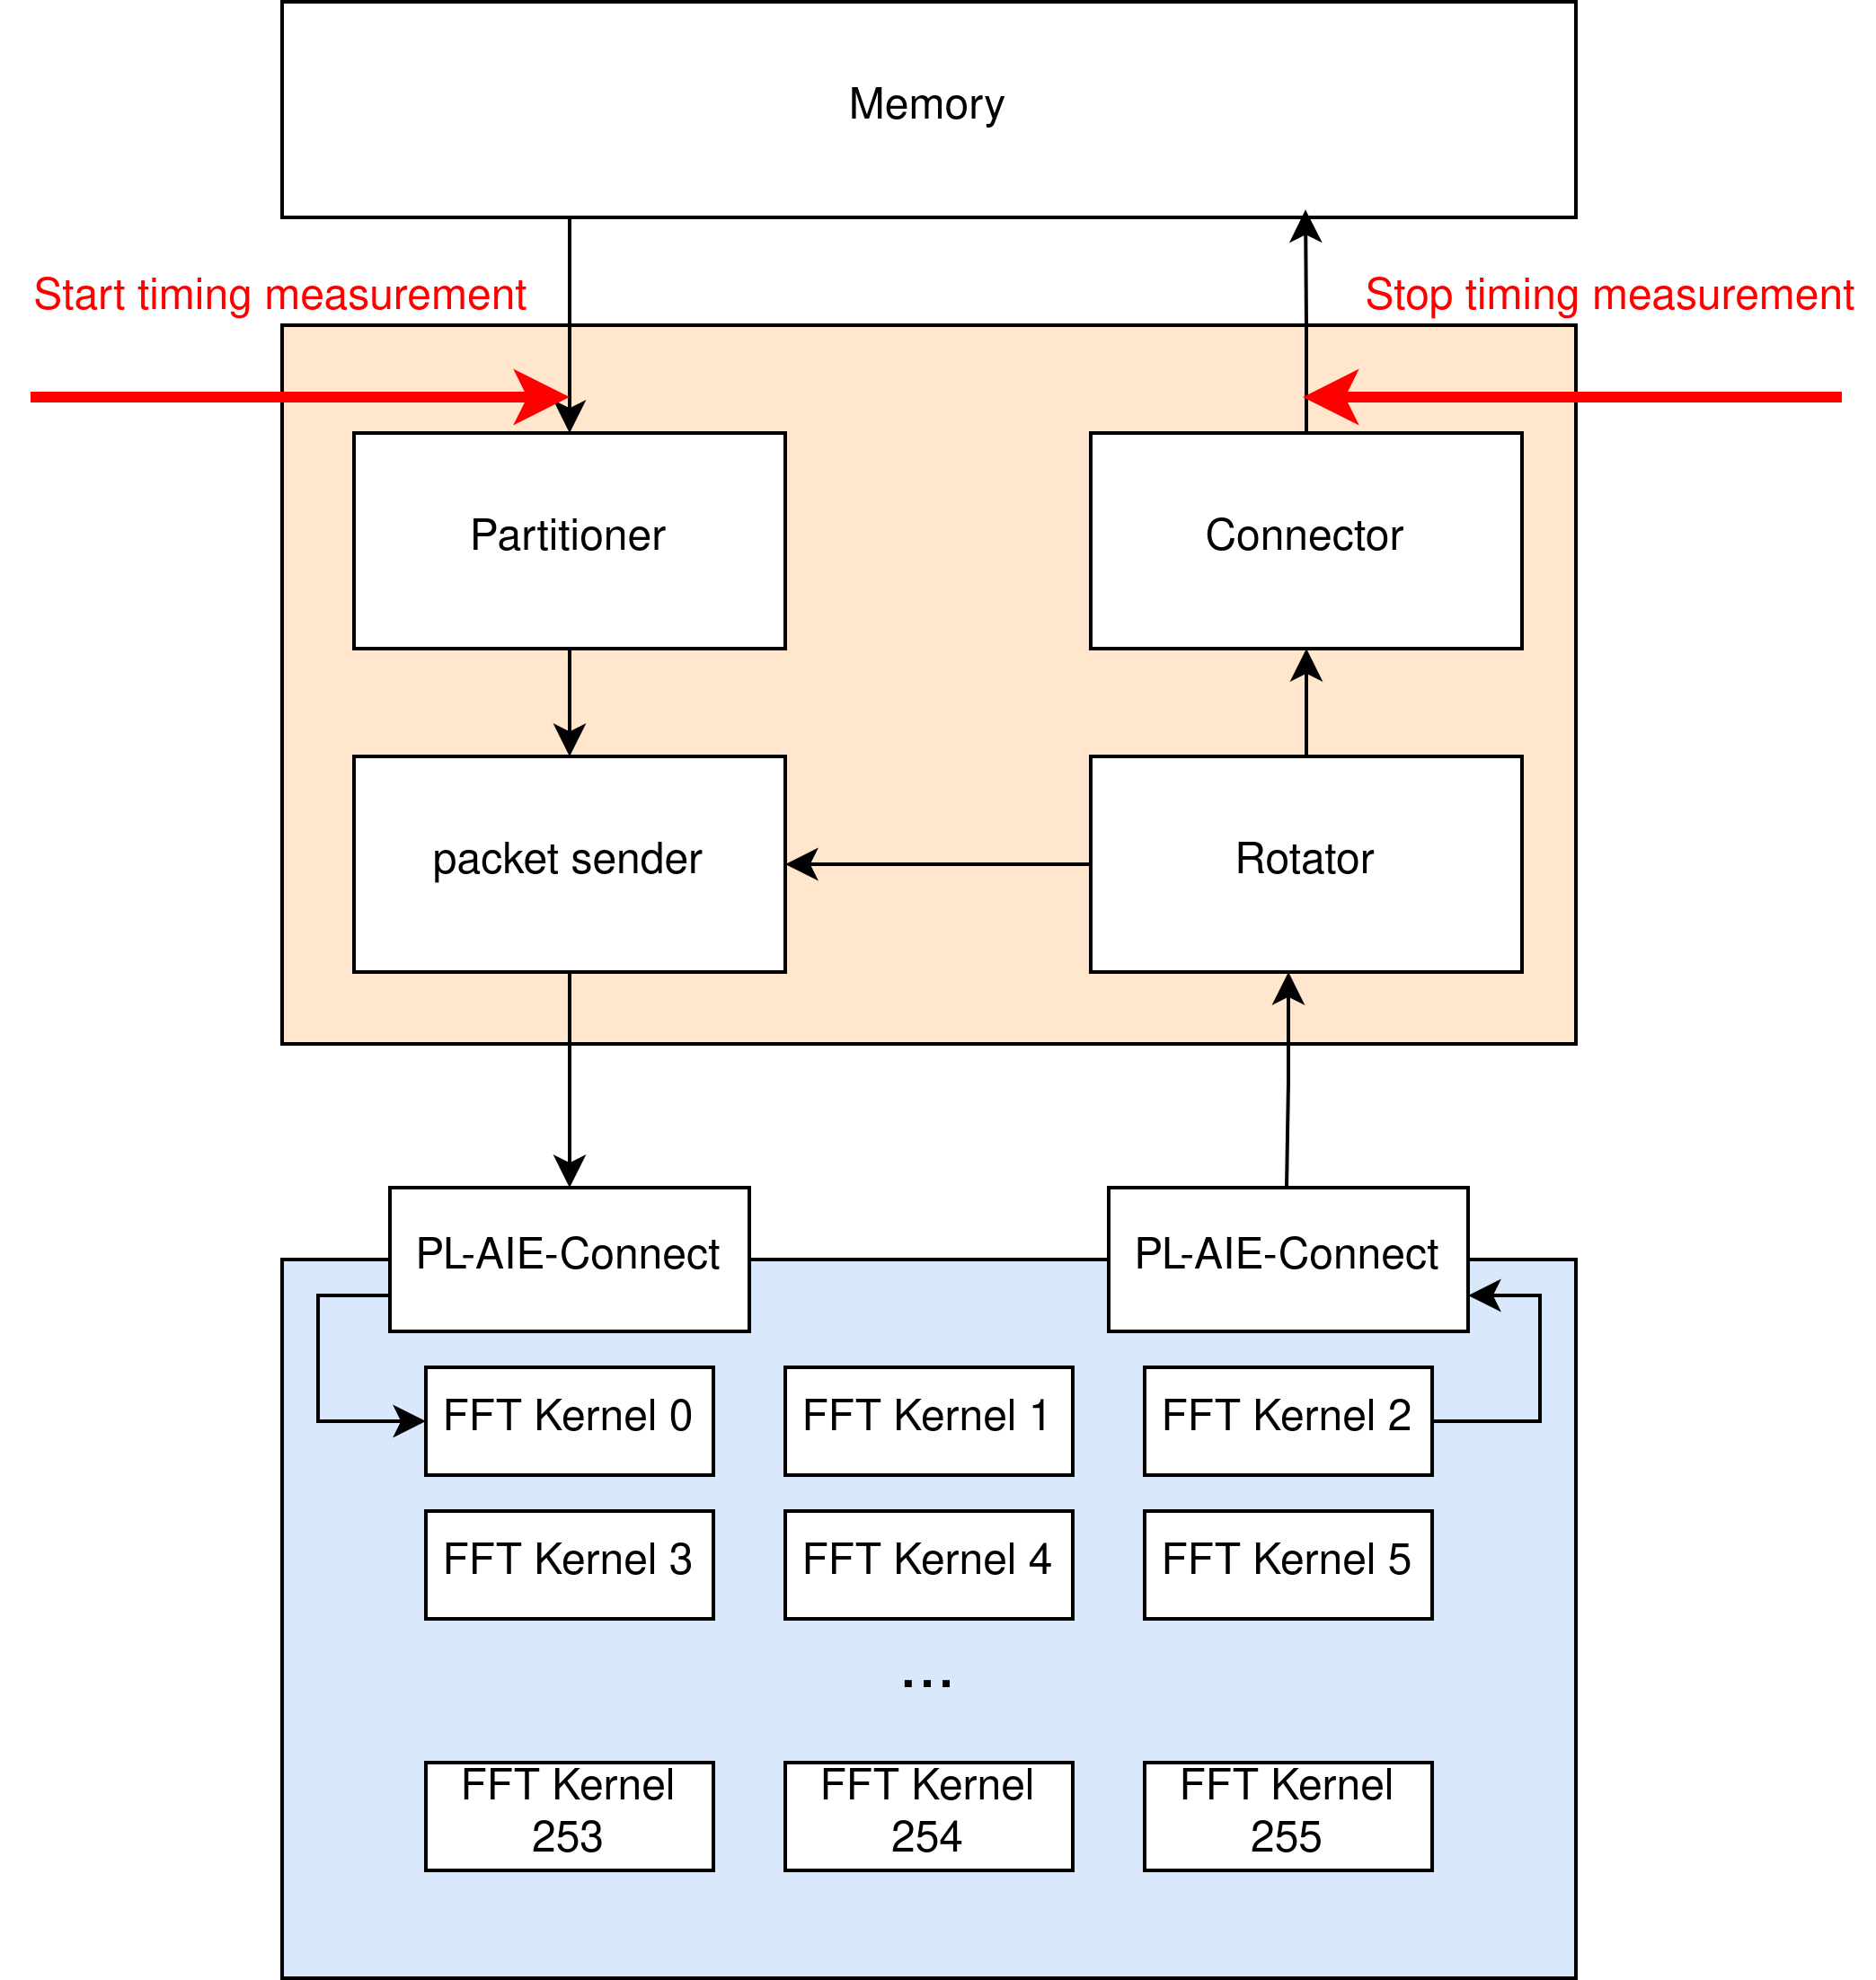
\includegraphics[width=0.6\textwidth]{images/timing.png}
    \captionsetup{justification=centering}
    \caption{Design with arrows which denotes the start and endpoint of the measurement}
    \label{fig:timing}
\end{figure}

Before presenting the results, I will briefly introduce the design choices under comparison. One of these choices is the streaming configuration of the AI Engines. There are two ways to implement streaming: the first is by reading each element from a stream and saving it to local memory, and the second is by allowing the stream to be automatically written to a predefined buffer, which is the approach used in the current design as described in section \ref{sec:aie_im}. Another important design aspect is the use of vector instructions for multiplications and additions, which could alternatively be implemented more simply on the scalar unit of the AI Engine core. Additionally, a key feature of the proposed design is the use of lookup tables for precomputed factors, so a version without this optimization will also be compared. The design further incorporates specialized load instructions for the vector units, and their impact on overall performance is also evaluated. Lastly, a comparison is made with the current complete prototype.

\section{Benchmark results}
Figure \ref{fig:plot1} illustrates the runtime performance for all test cases. To evaluate the precision of the proposed method, the root mean square error (RMSE) is also presented, with a defined threshold of -60 dB indicated by a red dotted line which was established as an acceptable error by Jensen et al. \cite{jens}. A green line at the end of the graph marks the real-time target for the algorithm. The aforementioned optimizations are applied incrementally. This means all improvements of the previous optimization step are carried over to the next which results in a ascending order of all steps in the performance diagram. In the bottom left, the naive implementation is shown, which displays a significant gap to the first optimization step. This gap is so substantial that part of the x-axis is truncated. This difference arises because the naive implementation processes each incoming stream element individually instead of buffering all elements at once. This method requires a memory instruction for each element, which not only increases the processing time per kernel but also introduces back pressure on the stream, as the stream processing time increases. This delay propagates through the entire array, resulting in a significant performance improvement when data is streamed directly into memory.\par
%TODO add plot from interime defense but with the final vector opt in the end; change the naming scheme according to this paragraph

\begin{figure}[h]
    \centering
    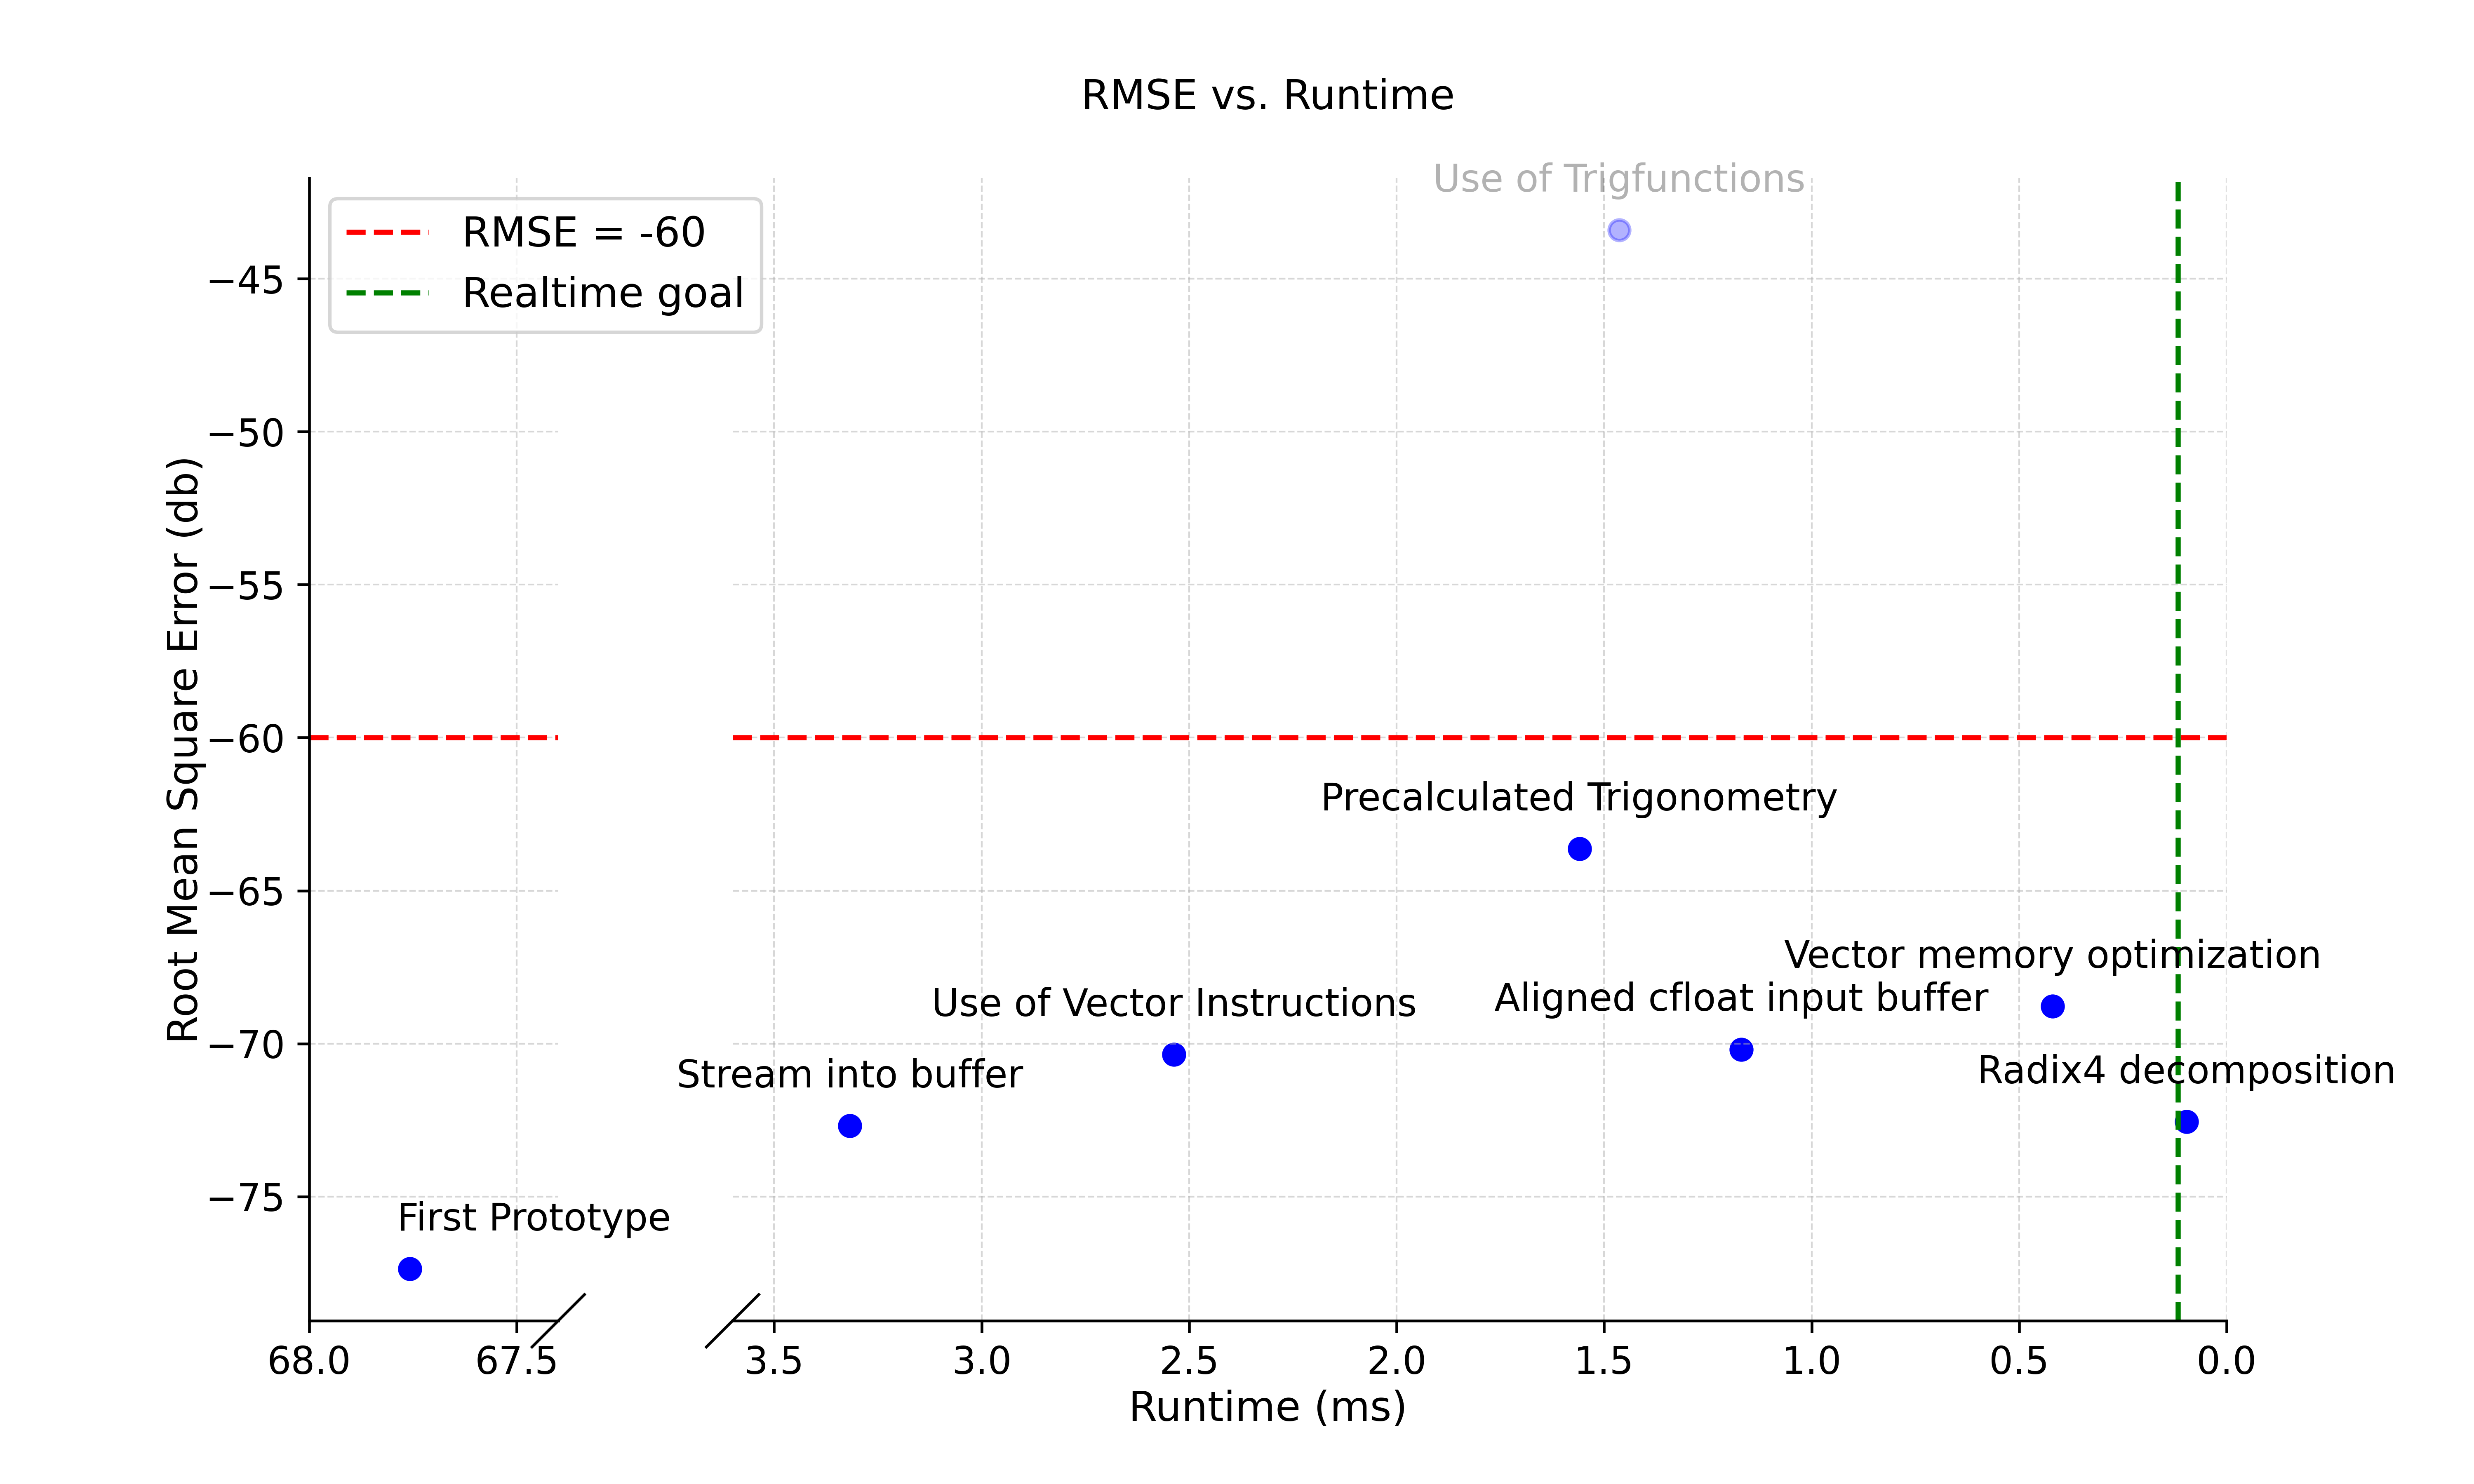
\includegraphics[width=0.9\textwidth]{images/simple_plot.png}
    \captionsetup{justification=centering}
    \caption{Various optimization steps with smaller prototype}
        Multiple iterative optimization steps in dependence from the root mean square error and the runtime. A break in the x-axis highlights the range of the runtime. The goal for realtime (green) and the maximum threshold for an error (red) are shown as dotted lines. 
    \label{fig:plot1}
\end{figure}

Figure \ref{fig:plot2} provides a different angle of the results, illustrating the different optimization steps based on the number of transformers that can be computed per second. The real-time target is again indicated by a green dotted line, assuming that 256 \ac{fft}s need to be completed within a 30 ms time frame, which equates to a real-time threshold of 8,524 \ac{fft}s per second. This representation highlights the significant performance increase achieved by utilizing the vector unit compared to all other optimizations.\par 
%TODO add throughput graph here and write paragraph about it

\begin{figure}[h]
    \centering
    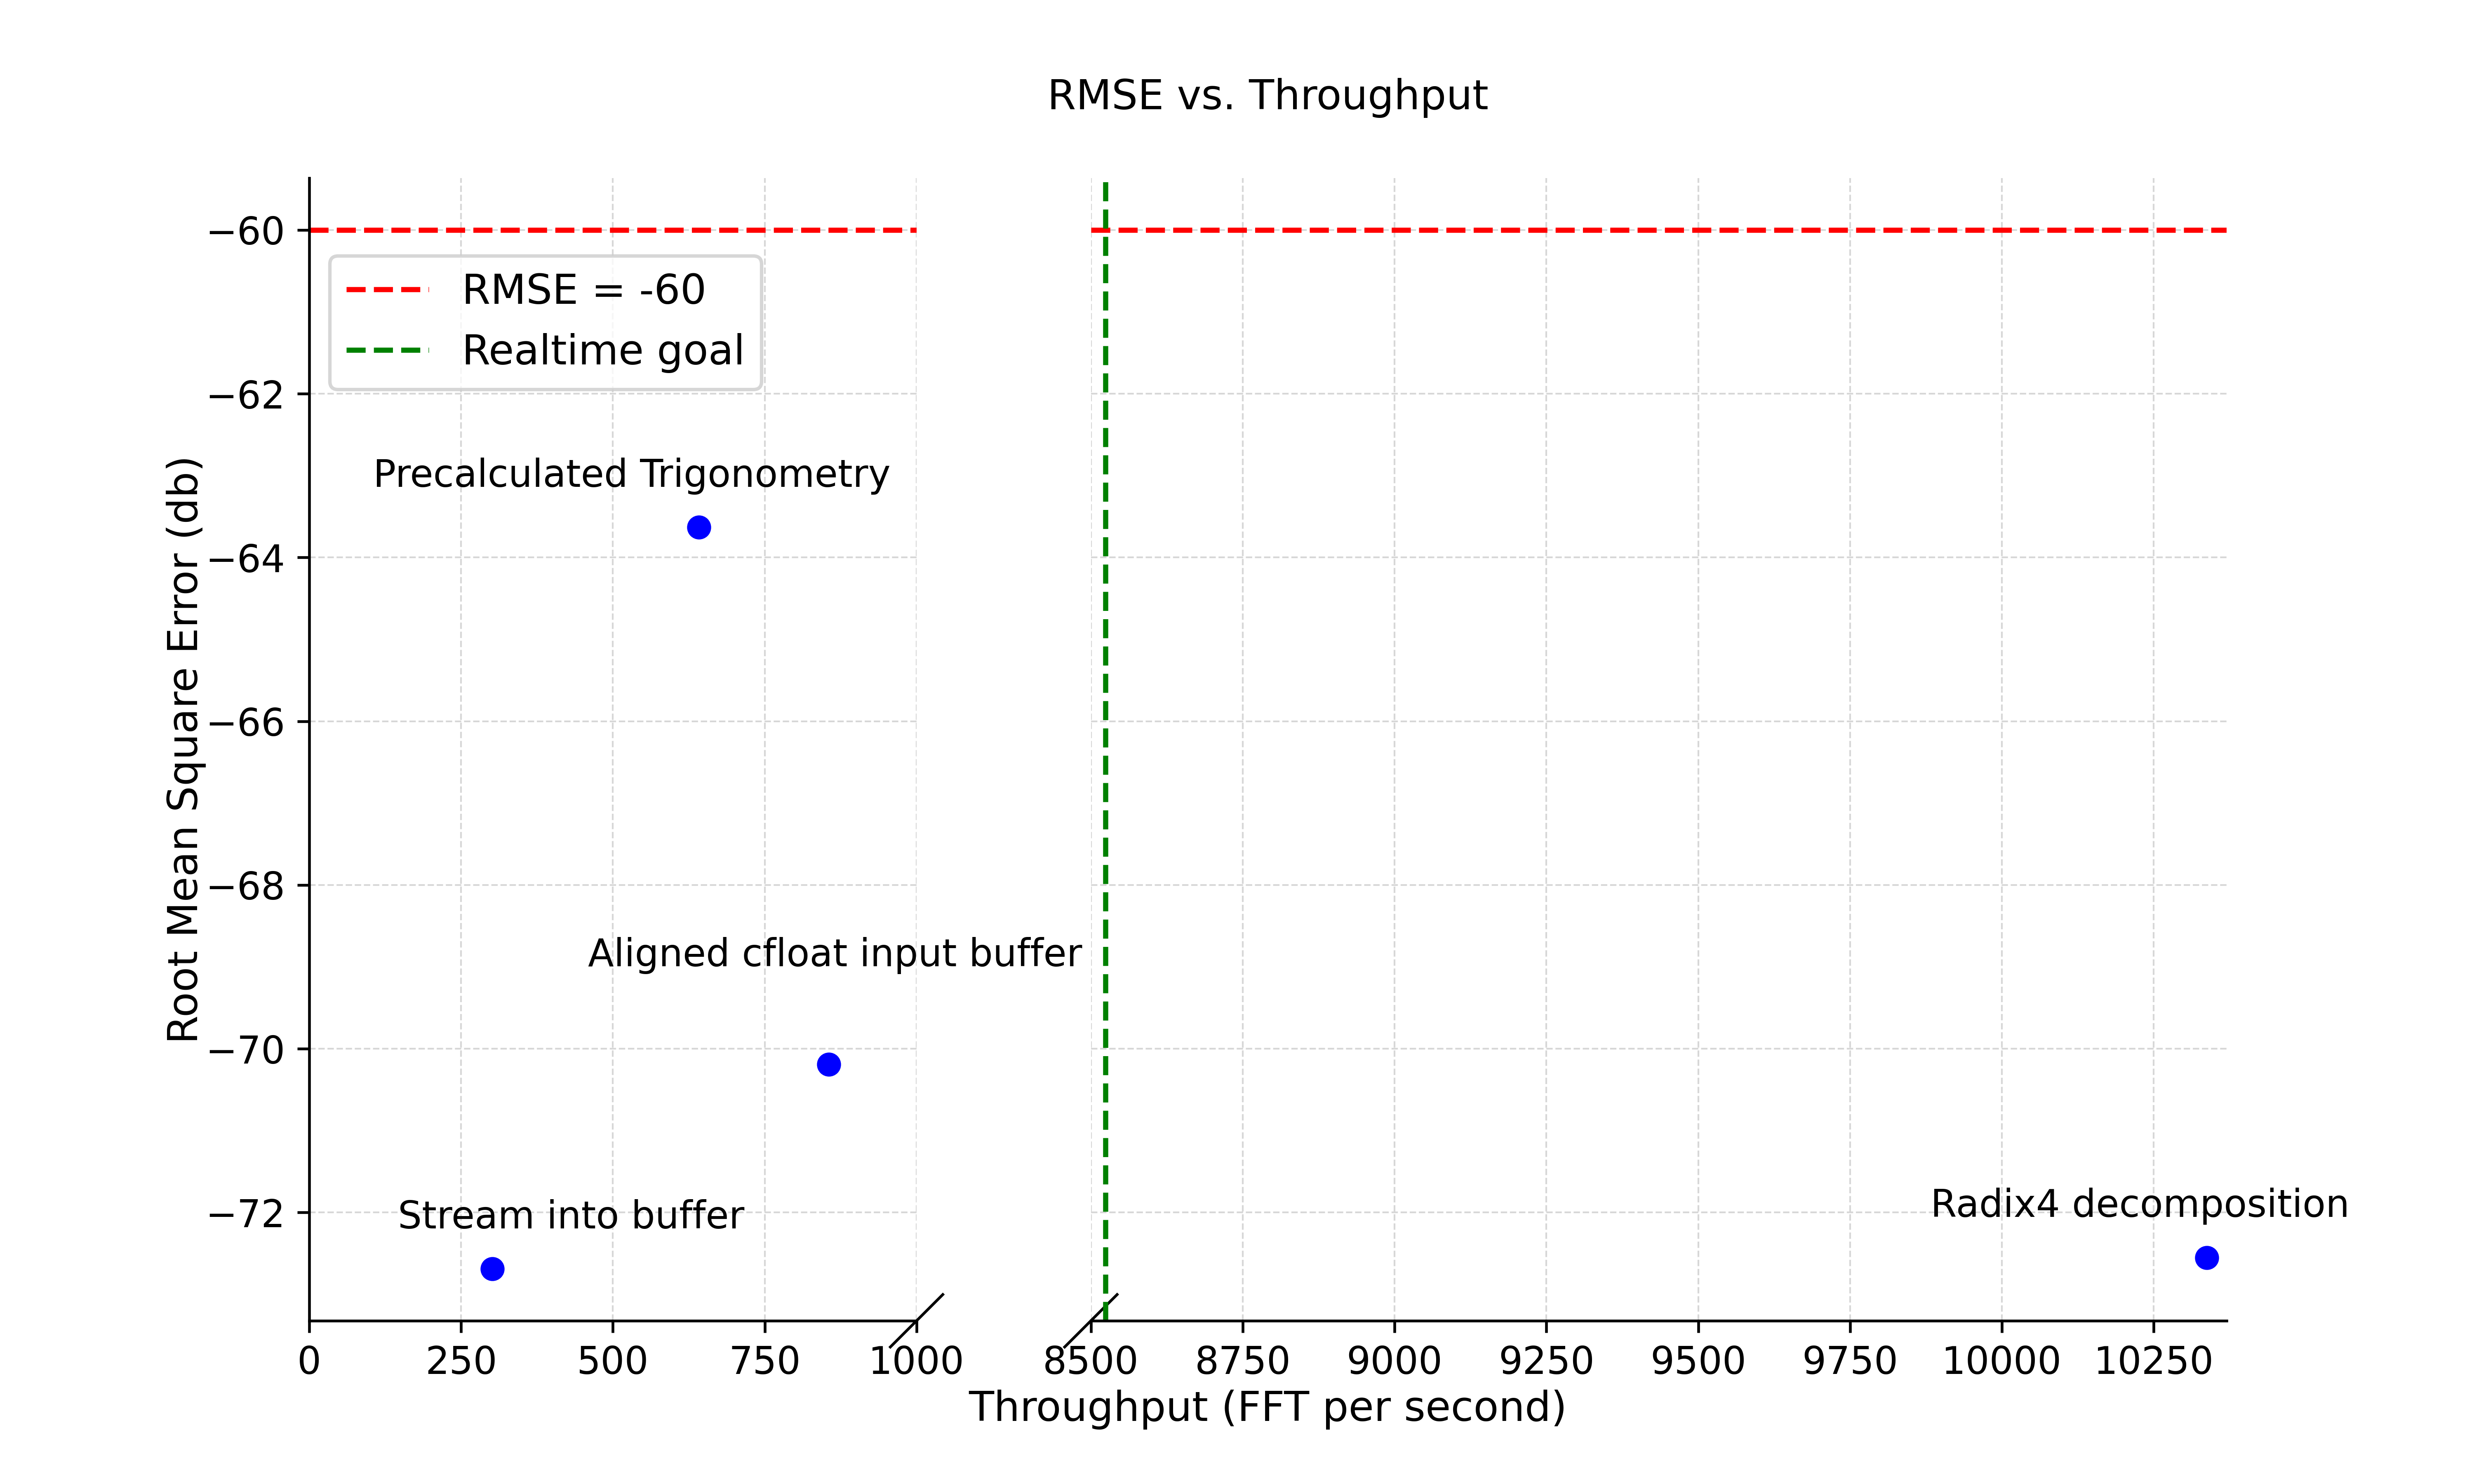
\includegraphics[width=0.9\textwidth]{images/throughput_plot.png}
    \captionsetup{justification=centering}
    \caption{Throughput of selected datapoints}
        A selection of iterative optimization steps in dependence from the error and the throughput. Through a break in the x-axis the huge difference between the optimization steps is highlighted.
    \label{fig:plot2}
\end{figure}

Another noteworthy aspect in this figure is the substantial difference in precision between using lookup tables and Xilinx-specific functions that calculate values at runtime. This discrepancy can be attributed to differences in the floating-point calculation units on the Versal platform versus the x86 processor, where values were precomputed. As shown, the precision of this method is still considerably lower than that of other optimizations and only improves when the lookup table and all other buffers are page-aligned. An analysis of the function trace revealed that this precision loss was due to a rounding function that was triggered each time a write-back occurred to a non-aligned memory location. By aligning the buffers, this precision loss was prevented. A beneficial side effect of this alignment was a reduction in runtime, as it enabled the use of faster memory access functions that operate only with aligned buffers, as described in section \ref{sec:aie_im}. The optimization using the proposed vector implementation ultimately enabled the algorithm to meet real-time requirements by reducing runtime below the real-time threshold.
%TODO add comparison in runtime between last optimization step and scale up to 262144 points

\begin{figure}[h!]
    \centering
    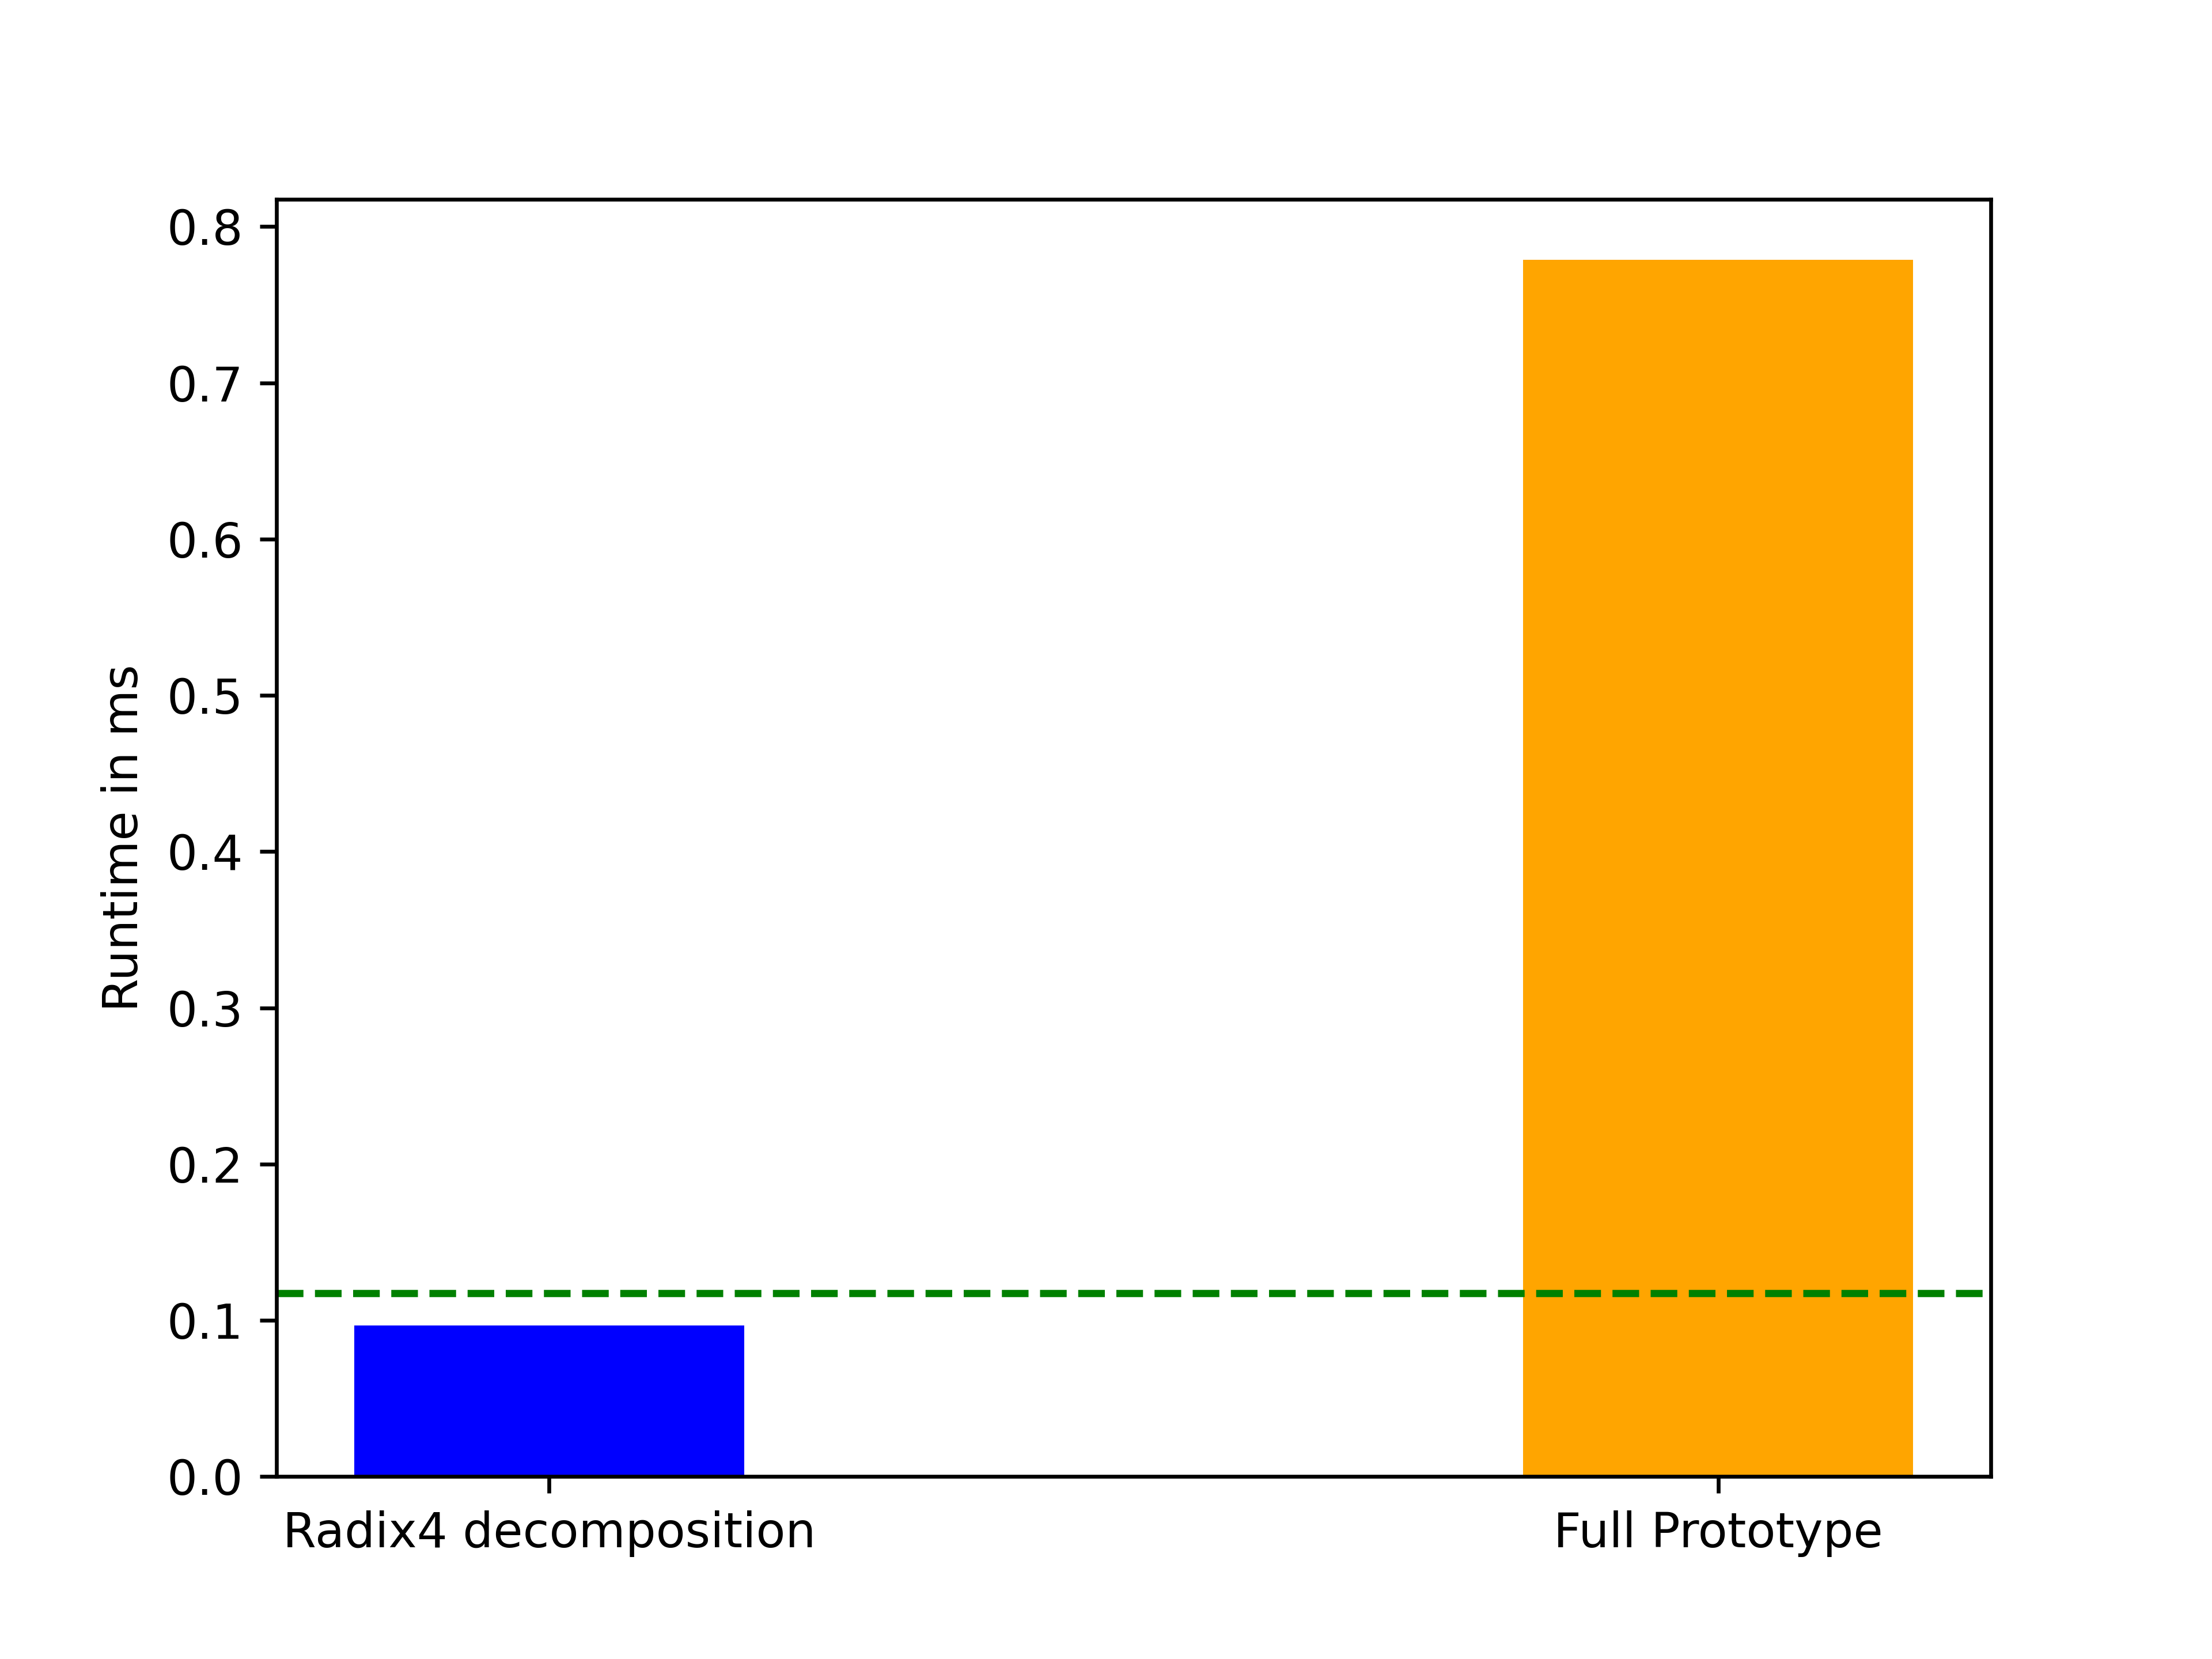
\includegraphics[width=0.6\linewidth]{images/bar_chart.png}
    \captionsetup{justification=centering}
    \caption{Comparison between the smaller and the larger prototype}
        This plot highlight the difference between a smaller prototype and the full $2^{18}$ prototype regarding runtime.
    \label{fig:last_stage}
\end{figure}
    
Figure \ref{fig:last_stage} presents a comparison between tests of a 32,768-point \ac{fft} and a $2^{18}$-point \ac{fft} using the proposed design which where both run on the previous described setup. It is evident that the larger \ac{fft} does not meet real-time requirements. To understand the source of this discrepancy, a closer examination of each component’s runtime is necessary. Figure \ref{fig:part_comp} breaks down the algorithm’s components and shows their respective runtimes, divided between the \ac{pl} and AI Engines kernels. The calculation time for the first stage exhibits a linear increase, which is expected, as the 1,024-point kernel in the $2^{18}$-point \ac{fft} uses four 256-point \ac{fft}s. Consequently, its runtime is approximately four times longer. The actual runtime is slightly higher due to additional memory management overhead and phase rotation after each 256-point \ac{fft}. The same pattern holds for the second stage kernel, which also uses four 256-point \ac{fft}s. Since this stage lacks phase rotation, its runtime aligns more closely to four times that of the smaller kernel. The noticeable gap between the second stage of the larger and smaller prototypes arises from the difference in second-stage kernel sizes, which is 128 points for the smaller prototype.\par

\begin{figure}[h]
    \centering
    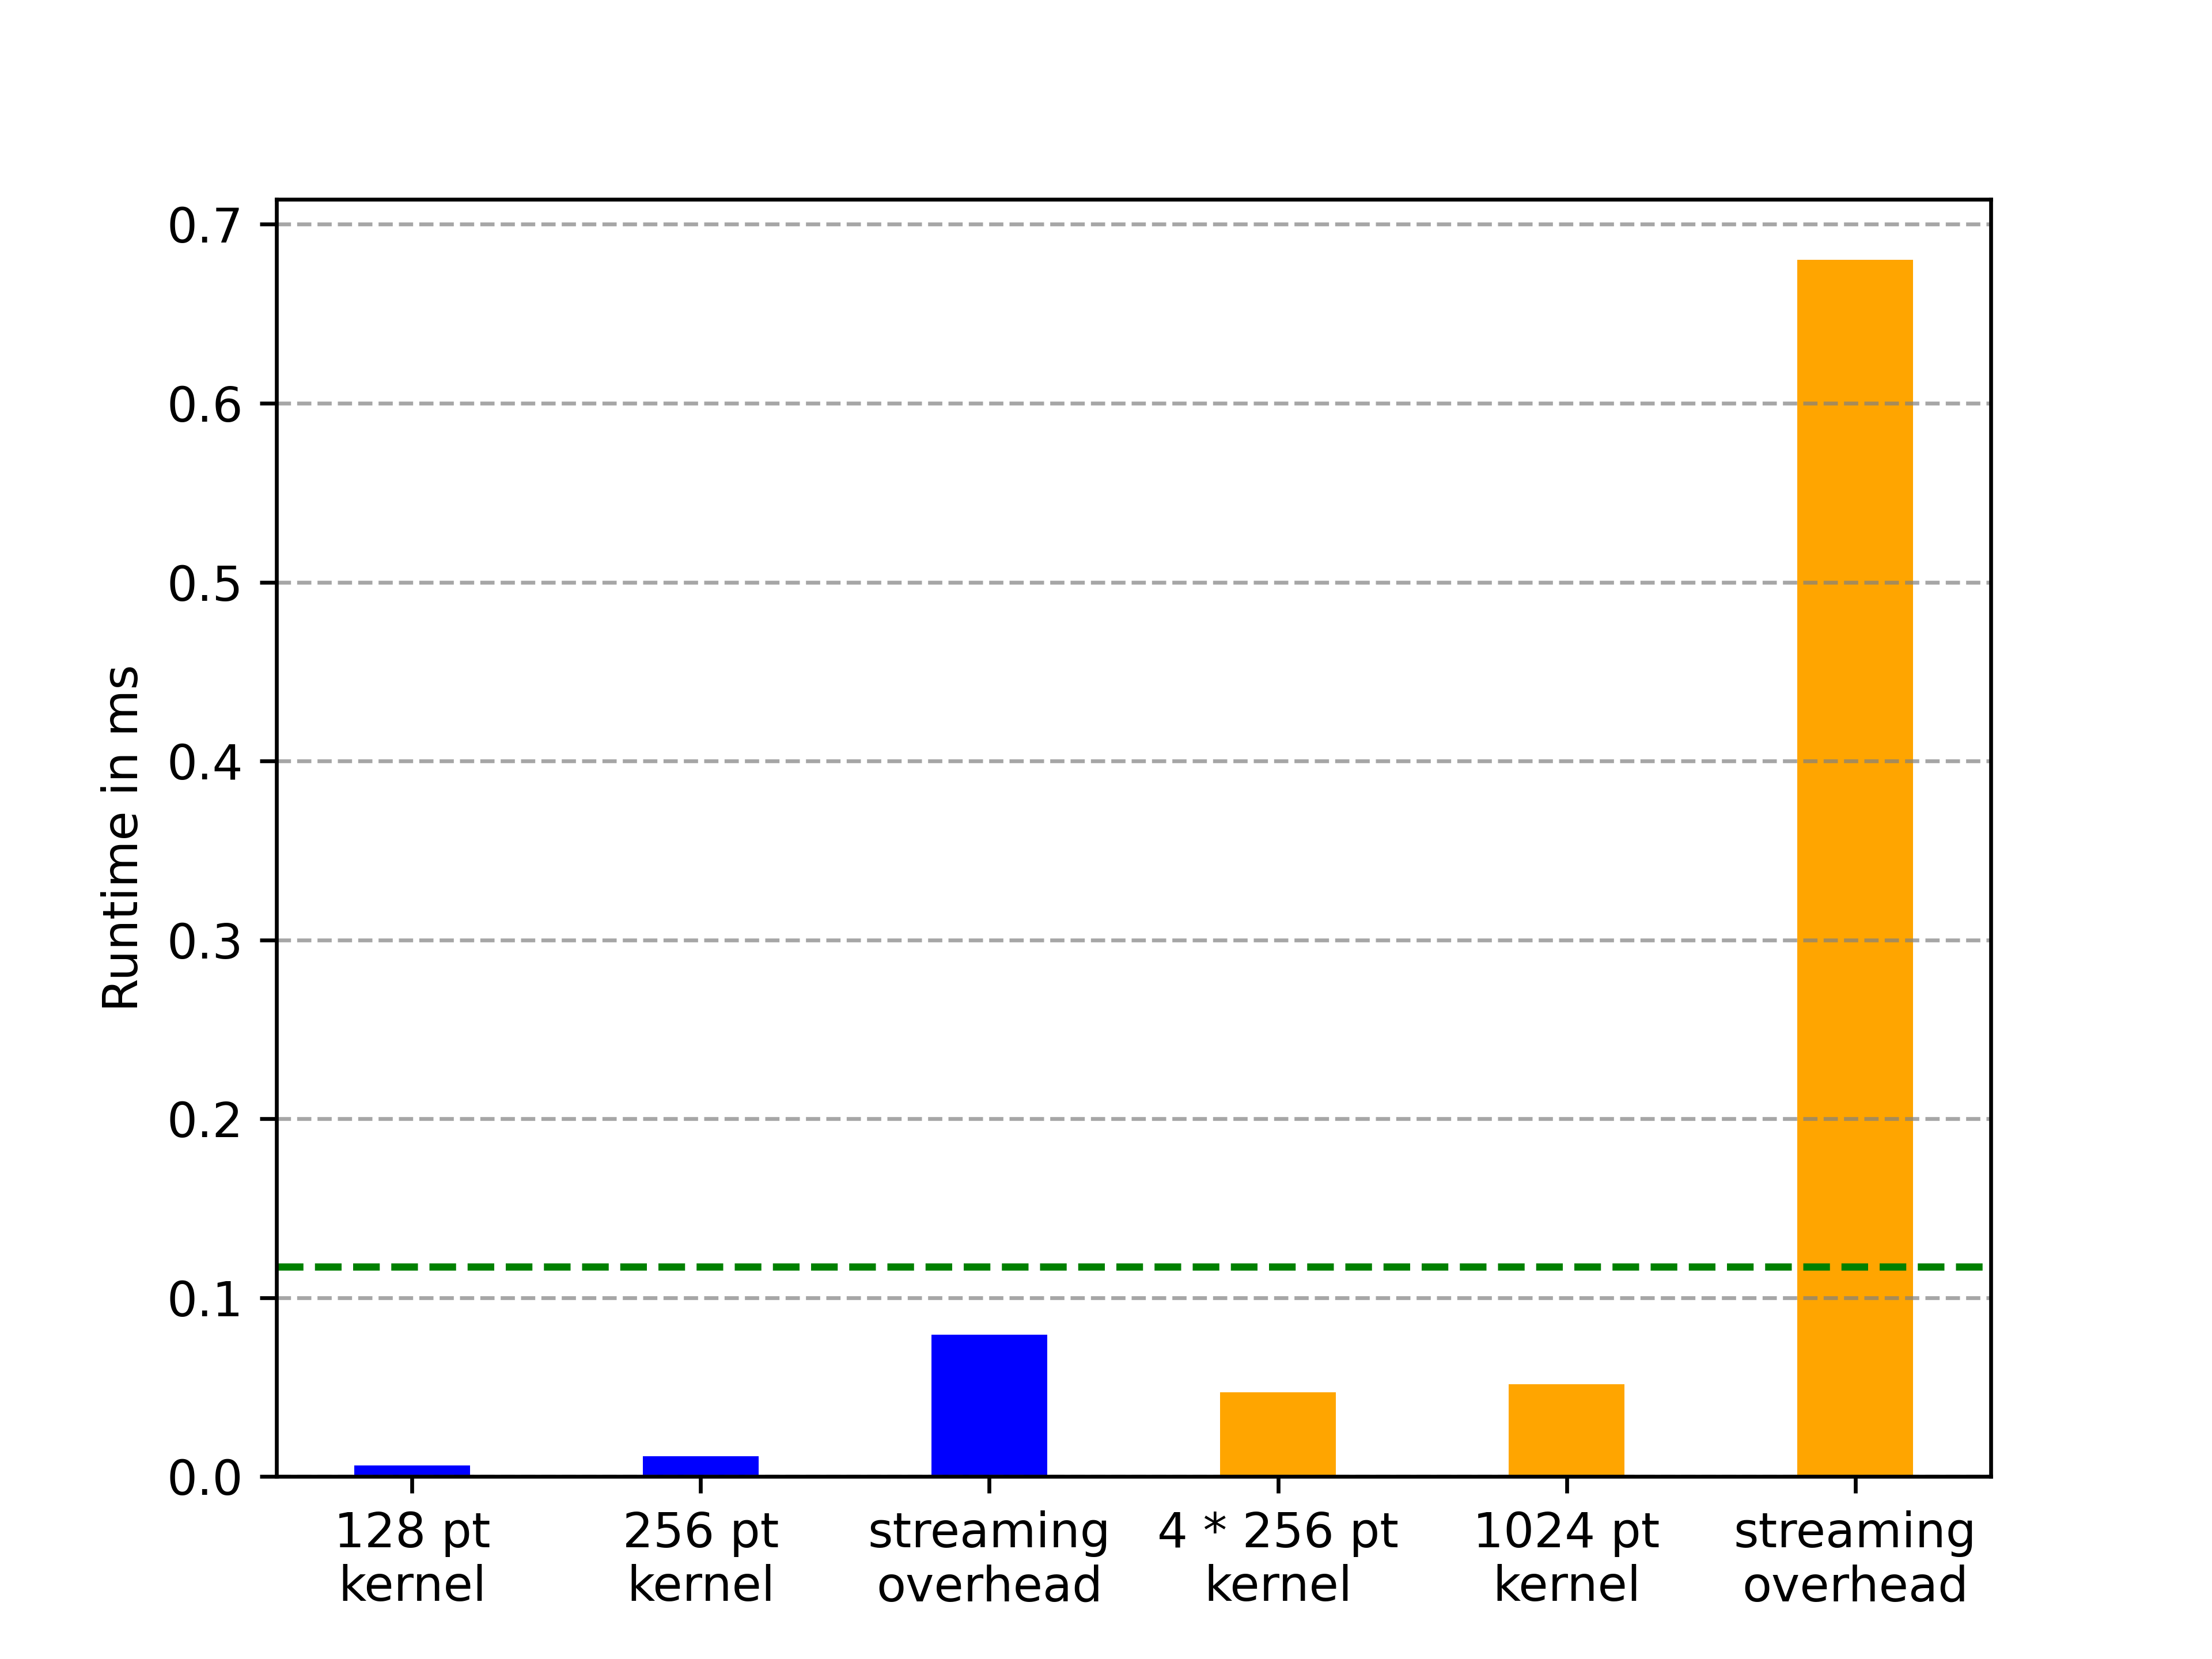
\includegraphics[width=0.6\linewidth]{images/part_comp.png}
    \captionsetup{justification=centering}
    \caption{Comparison between different stages of the algorithm}
        By splitting both, the smaller and the larger prototype, into there specific parts during runtime measurements the significant overhead of the data streaming is highlighted.
    \label{fig:part_comp}
\end{figure}

However, the most critical finding in this analysis is the time spent on streaming within the \ac{pl}. While the calculation time remains well below the real-time threshold, the interval between the first and second stages of the algorithm exceeds this limit by nearly sixfold. Several factors contribute to this issue. One is the clock frequency difference: the \ac{pl} runs at 200 MHz, whereas the AI Engines operates at 1250 MHz, leading to increased synchronization overhead between these hardware layers. This frequency mismatch also reduces the number of operations executable within a given timeframe. Additionally, the simple design of the \ac{pl}, coupled with a high-level synthesis approach where much of the implementation relies on compiler-generated code \cite{huang_survey_2020}, can result in significant underutilization of available resources.
%TODO add figure with time spend at which part of the FFT